\chapter{Project Organisation}
\label{ch:proj_orga}
%checked by Bryan @2102

A team must have a solid team structure such that team members can work at maximum efficiency. After defining and distributing tasks, team rules need to be formulated for managing the team. In addition, the work must be approached in a structured manner, therefore a work flow and schedule must be created.

The team structure and organisation management are elaborated in \autoref{sec:orga_struc}, whilst the Work Flow Diagram (WFD), Work Breakdown Structure (WBS), and the Gantt chart are shown in \autoref{sec:work_appr}. 


\section{Organisational Structure}
\label{sec:orga_struc}
In this section, the non-technical and technical tasks will be described and assigned to each team member. Relations between tasks can be found in an organogram.

\subsection{Organogram}

The organogram of the team can be seen in \autoref{fig:organogram}. 
The organogram is divided into a management department, an engineering department and a chairman. 
The engineering department is responsible for designing a product or a system. It consists of specialised units as following: cost engineers, reliability engineers, performance engineers, control \& stability engineers, sustainability engineers, ground handling engineers and risk engineers.
The management department mainly manages the team and organisational tasks. It consists of a time manager, a secretary, administrators, a sustainability manager, quality control managers and system engineers. The chairman connects the engineering and management departments with great communication skills and a solid overview of project phases in both organisational and technical aspects.


\begin{figure}[H]
    \centering
    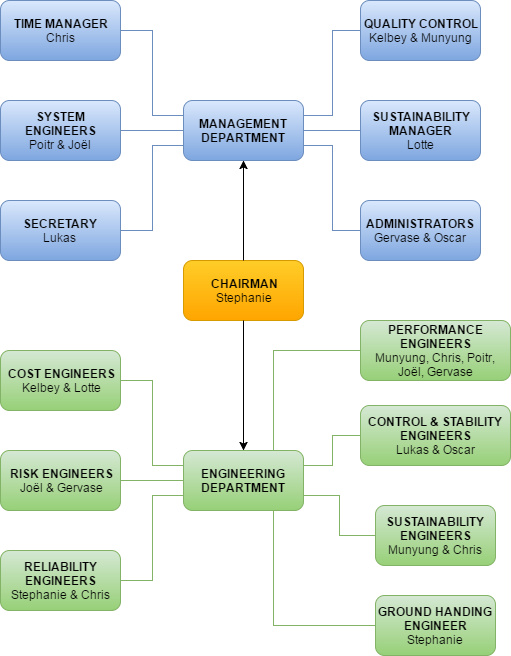
\includegraphics[width=0.5\textwidth]{ProjectOrganisation/Figures/Organogram}
    \caption{Organisational breakdown structure}
    \label{fig:organogram}
\end{figure}

\subsection{Non-Technical Task Division}
Description and distribution of non-technical tasks for corresponding roles can be seen in \autoref{tab:nttdiv}.

\begin{table}[H]
    \centering
    \caption{Description and distribution of the non-technical tasks within the team}
    \label{tab:nttdiv}
    \begin{tabular}{p{2.7cm}lp{10cm}}
        \toprule \
        \textbf{Role}      & \textbf{Name}     & \textbf{Assigned Tasks} \\
        \toprule \
        Chairman & Stephanie & - Leads meetings \\
         &  & - Is a contact person for external communication \\
         &  & - Has broad overview of overall progress and group dynamics \\
         &  & - Monitors the functioning of the organisation \\
         &  & - Takes action when the organisation or individuals perform sub-optimal on non-technical tasks \\ \hdashline
        Quality Control & Munyung & - Check lingual consistency of the report \\
                        & Kelbey & - Check compliance with writing procedures \\
         &  & - Resolve latex syntax errors \\
         &  & - Check spelling and grammar \\
         &  & - Check if deliverables are present \\ 
         &  & - Develop a quality control system \\ \hdashline
        Secretary & Lukas & - Makes notes during internal and external meetings \\
         &  & - Documents action points and questions for coaches and/or project supervisor \\ \hdashline
        Systems & Piotr & - Make sure that SE tools are being implemented correctly \\
        Engineer         &  Joël & - Make sure that SE tools are used throughout the project \\
        &  & - Make sure that SE tools are being updated continuously \\ \hdashline
        Time Manager & Chris & - Keeps track of the planning \\
                     &       & - Makes sure that the task management system (Trello) is up to date \\
         &  & - Spots delays early on \\
         &  & - Communicates with chairman to minimize further delays by reallocating human resources \\ \hdashline
        Sustainability & Lotte & - Monitors the overall sustainability of the design \\
        Manager &   & - Brings sustainability to the attention of the subsystem designers \\
         &  & - Ensures that the strategy for manufacturing, support and end-of-life solution of the product are sustainable \\ \hdashline
        Administrators & Oscar & - Structure and monitor file directories \\
         & Gervase & - Oversee the product data management system \\
         &  & - Implement changes in the master document \\
         &  & - Keep track of released versions of documents \\ \bottomrule
    \end{tabular}
\end{table}

\subsection{Technical Task Division}
Description and distribution of technical tasks for corresponding roles can be seen in \autoref{tab:ttdiv}. A division by trade-off criteria is chosen instead of a division by concepts, since it is efficient for team members to research one technical domain and apply it to each concept. Furthermore, biased analysis can be avoided, as team members cannot apply their preferences to analysis of a specific concept when tasks are divided based on criteria. 

The technical roles are included in the engineering department in the organogram.

\begin{table}[H]
    \centering
    \caption{Distribution and Description of Technical Tasks}
    \label{tab:ttdiv}
        \begin{tabular}{>{\raggedright\arraybackslash}p{3.5cm}>{\raggedright\arraybackslash}p{3.5cm}>{\raggedright\arraybackslash}p{7cm}}
        \toprule 
        \textbf{Role} & \textbf{Name} & \textbf{Assigned Tasks} \\ \toprule
        Performance engineers & Munyung, Chris, Poitr, Joël, Gervase & Analyse performance of each concept in terms of range, endurance, mass, drag and power required for max speed, climb rate and hovering \\
        \hdashline
        Sustainability engineers & Munyung, Chris & Evaluate sustainability of each concept in terms of noise emission and manufacturing sustainability\\
        \hdashline
        Cost engineers & Kelbey, Lotte & Evaluate production cost of each concept in terms of manufacturing cost, material cost, mechanism cost, propulsion \& power cost and influence of weight on cost\\ 
        \hdashline
        Reliability engineers & Stephanie, Chris & Assess reliability of control surfaces, wings and propulsion systems for each concept\\ 
        \hdashline
        Risk engineers & Joël, Gervase & Assess risk of each concept in terms of feasibility, complexity and available expertise\\ 
        \hdashline
        Control \& stability engineers & Oscar, Lukas & Evaluate each concept based on control, stability and manoeuvrability\\ 
        \hdashline
        Ground handling engineer & Stephanie & Evaluates ground handling of each concept in terms of assembly the UAV, dimensions, mass, payload mounting and maintenance \\
        \bottomrule
    \end{tabular}
\end{table}

\begin{comment}
\subsection{Non-Technical Task Division}
Description and distribution of non-technical tasks for corresponding roles can be seen in \autoref{tab:nttdiv}.

\begin{table}[H]
    \centering
    \caption{Description and distribution of the non-technical tasks within the team}
    \label{tab:nttdiv}
    \begin{tabular}{p{2.7cm}lp{10cm}}
        \toprule \
        \textbf{Role}      & \textbf{Name}     & \textbf{Assigned Tasks} \\
        \toprule \
        Chairman & Stephanie & - Leads meetings \\
         &  & - Is a contact person for external communication \\
         &  & - Has broad overview of overall progress and group dynamics \\
         &  & - Monitors the functioning of the organisation \\
         &  & - Takes action when the organisation or individuals perform sub-optimal on non-technical tasks \\ \hdashline
        Quality Control & Munyung & - Check lingual consistency of the report \\
                        & Kelbey & - Check compliance with writing procedures \\
         &  & - Resolve latex syntax errors \\
         &  & - Check spelling and grammar \\
         &  & - Check if deliverables are present \\ 
         &  & - Develop a quality control system \\ \hdashline
        Secretary & Lukas & - Makes notes during internal and external meetings \\
         &  & - Documents action points and questions for coaches and/or project supervisor \\ \hdashline
        Systems & Piotr & - Make sure that SE tools are being implemented correctly \\
        Engineer         &  Joël & - Make sure that SE tools are used throughout the project \\
        &  & - Make sure that SE tools are being updated continuously \\ \hdashline
        Time Manager & Chris & - Keeps track of the planning \\
                     &       & - Makes sure that the task management system (Trello) is up to date \\
         &  & - Spots delays early on \\
         &  & - Communicates with chairman to minimize further delays by reallocating human resources \\ \hdashline
        Sustainability & Lotte & - Monitors the overall sustainability of the design \\
        Manager &   & - Brings sustainability to the attention of the subsystem designers \\
         &  & - Ensures that the strategy for manufacturing, support and end-of-life solution of the product are sustainable \\ \hdashline
        Administrators & Oscar & - Structure and monitor file directories \\
         & Gervase & - Oversee the product data management system \\
         &  & - Implement changes in the master document \\
         &  & - Keep track of released versions of documents \\ \bottomrule
    \end{tabular}
\end{table}
\end{comment}

\begin{comment}
\section{Basic Team Rules and Agreements}

In order to streamline work processes of the team, basic agreements are made in the start-up phase of the project. A general daily working schedule is drafted to facilitate stability and routine. Additionally, a set of rules is agreed among team members in order to regulate the functioning of the team.

\subsection{Rules}
The following set of rules are agreed upon by the entire team during a first internal meeting.
\iffalse
\begin{enumitem}
    \item Everyday an internal meeting will be held at five o'clock in the afternoon at a reserved meeting room.
    \item Every Wednesday a meeting with the project coaches and mentor will take place at eleven o'clock at a predetermined location.
    \item The daily schedule (\autoref{tab:schedule}) shall be followed by the entire group.%The daily schedule dictates the breaks that the group can take throughout the day. It consists of two fifteen-minute coffee breaks (one at 1100 hours and one at 1530 hours), and one 30-minute lunch break at 1230 hours. Changes can be made on a daily basis in agreement with the entire team only.
    \item All team members will frequently report on the progress of their tasks via Trello, a web-based task monitoring tool.
    \item Each session starts at nine o'clock sharp. Being late to a session will have consequences. In the event that a member of the team arrives with a delay of more than ten minutes, the corresponding drop in morale has to be compensated for the next day. This will be in the form of a cake or pastry provided by the person in question.    
\end{enumitem}
\fi 

\subsection{Daily Schedule}
%The daily working schedule is shown in \autoref{tab:schedule}. In general, a working day will last from nine o'clock in the morning up until six o'clock in the evening. Throughout the day three breaks will take place with a total duration of one hour. The morning and afternoon will both have one fifteen minute coffee break with the lunch break in between these two. Additionally, two internal meetings are scheduled to take place everyday. This will be one short kick-off meeting to start the day with and a longer meeting in a reserved meeting room at five.

The daily working schedule is shown in \autoref{tab:schedule}. A working day will last from 0900 hours till 1800 hours. Throughout the day three breaks will take place; two fifteen-minute coffee breaks (one at 1100 hours and one at 1530 hours), and one 30-minute lunch break at 1230 hours. Additionally, two internal meetings are scheduled to take place everyday; one kick-off meeting to start the day, and one longer meeting in a reserved meeting room at 1700 hours.

\begin{table}[H]
\centering
\caption{Daily schedule}
\label{tab:schedule}
\begin{tabular}{ll}
\toprule
\textbf{Time} & \textbf{Activity} \\
\toprule
09:00-09:15 & Start with kick-off meeting \\
11:00-11:15 & First coffee break \\
12:30-13:00 & Lunch break \\
15:30-15:45 & Second coffee break \\
17:00-18:00 & Internal meeting \\
\bottomrule
\end{tabular}
\end{table}

\subsection{General Writing Rules}
In this section, some general writing rules are presented for formatting and typing in \LaTeX. This is done to ensure unity in the report and save quality control some time. 

\subsubsection{Referencing and Labelling}
Any label for a chapter, section, subsection, table and figure will start with ch:, sec:, sec:, tab: and fig: respectively. For chapter and section labels, the first four letters of each word of the title will be used to make referencing easier. Any referencing should be done using \texttt{autoref} in order to ensure consistency in the labels. The captions on Figures go below the Figures, the captions on tables go above the tables. These captions never end with a dot, and only the first letter is capitalised. The titles of chapters and sections should always be fully capitalised, except for the connection words. 

\subsubsection{Use of Abbreviations}
When using abbreviations, the full words should be spelt out at first use and should be mentioned in the list of abbreviations. This shall be done in the following format: 'This is the first time Use Of Abbreviations (UOA), is mentioned. Mentioning UOA later can be done in abbreviated form'.

\subsubsection{Tables}
In order to keep up the same appearance for all tables, use the commands \texttt{tabularx} to ensure size, and \texttt{toprule}, \texttt{midrule}, \texttt{bottomrule}, and \texttt{hdashline} to create the horizontal lines. No vertical lines are allowed.

\end{comment}

\section{Work Approach}
\label{sec:work_appr}
In this section, the revised WFD, WBS, and Gantt chart are shown below. The current project phase is portrayed in the third row in the WFD, and the third column in the WBS. 

\newpage

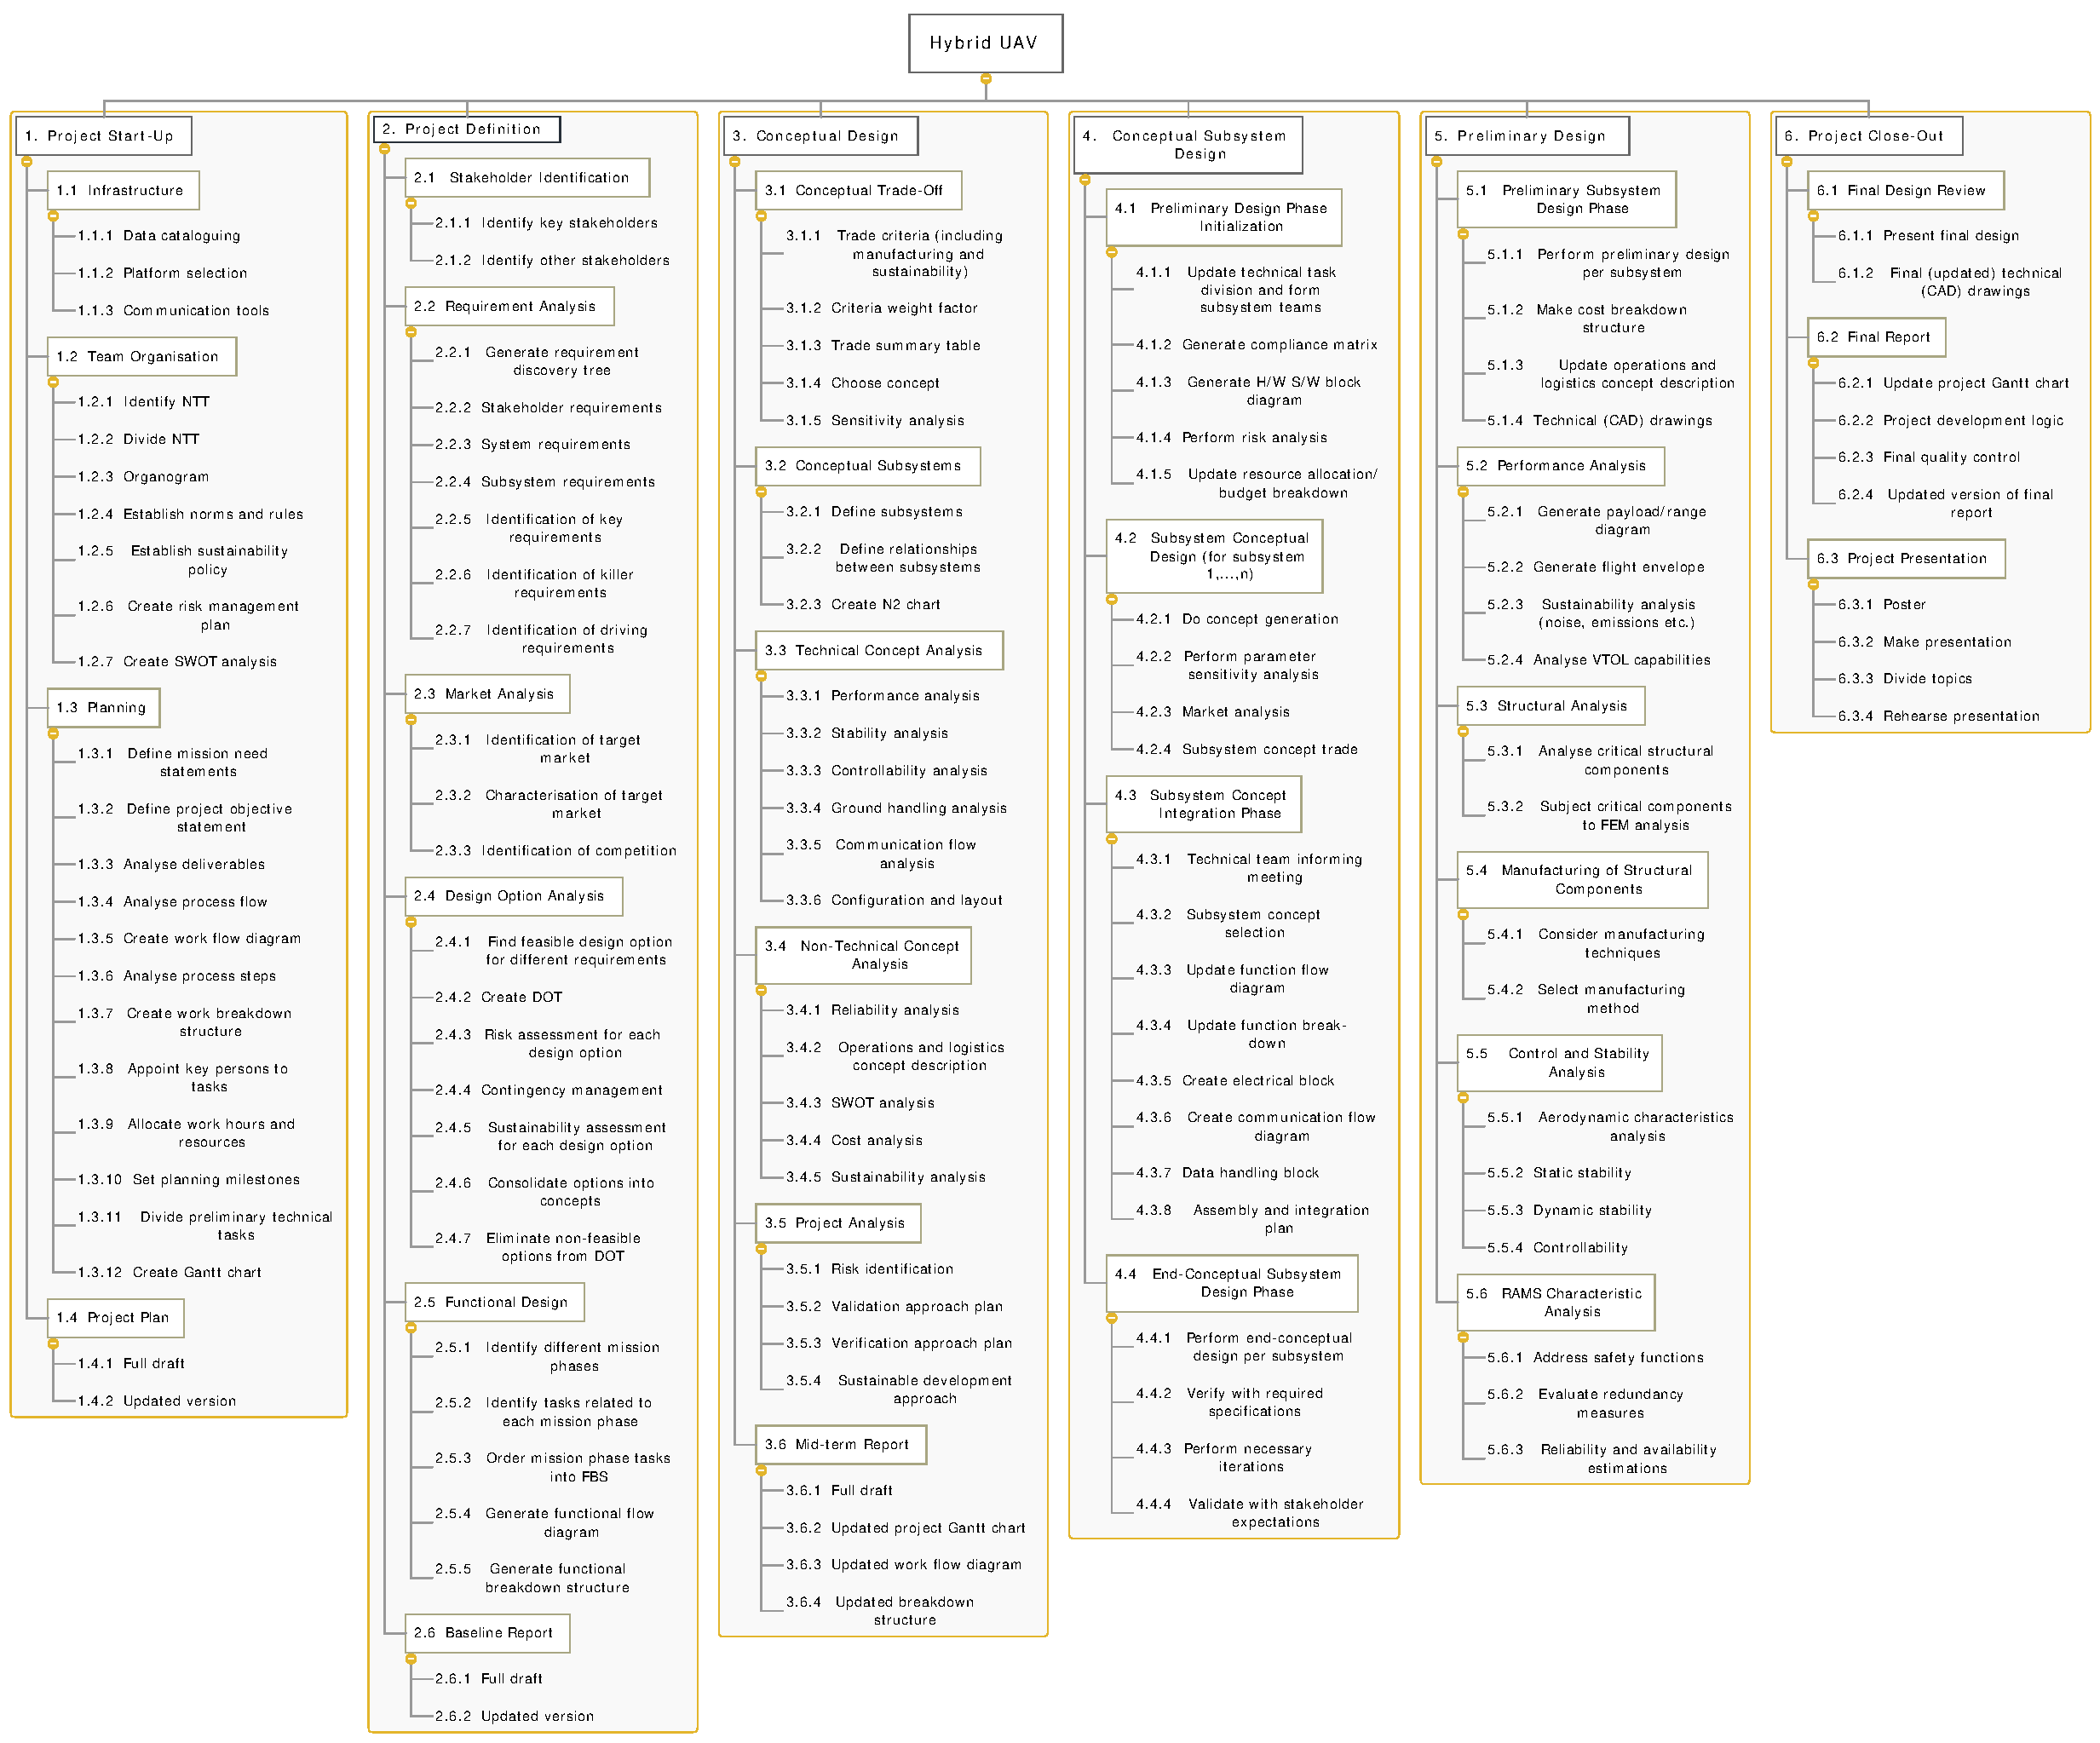
\includepdf[pages=1,fitpaper, scale=0.85,pagecommand={}]{ProjectOrganisation/Figures/WBS.pdf}

\newpage

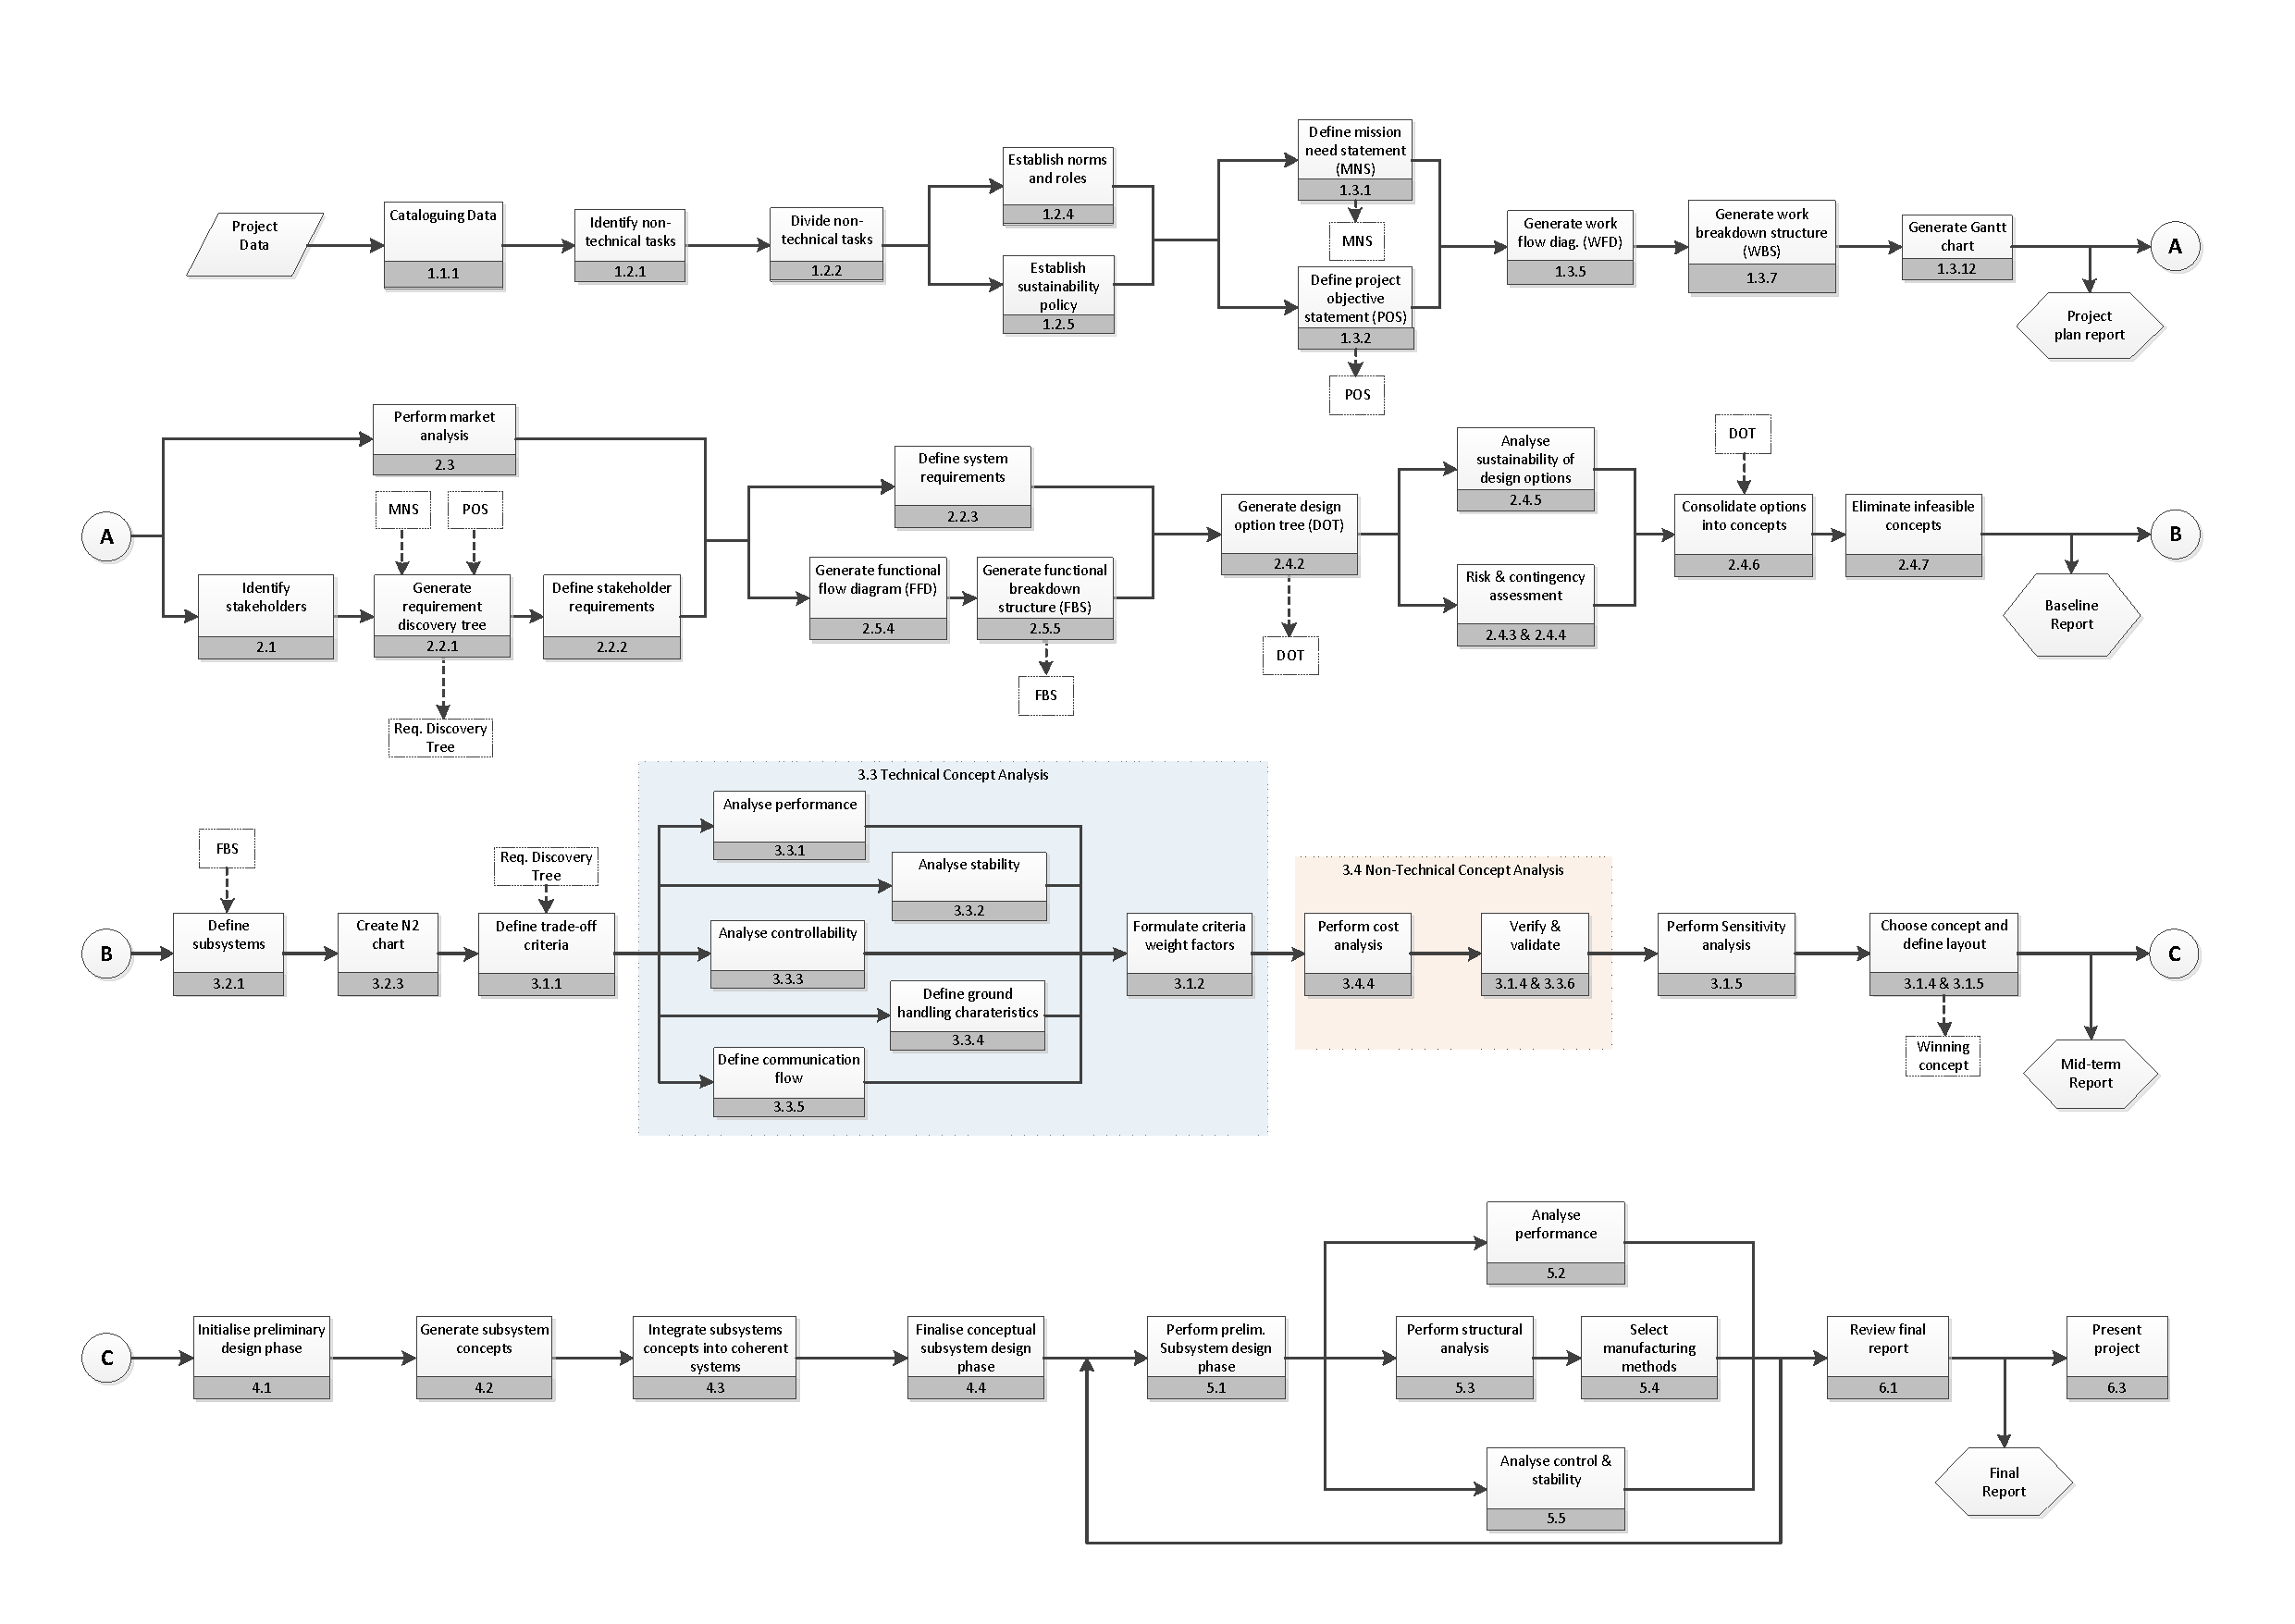
\includepdf[pages=1,fitpaper, scale=0.85,pagecommand={}]{ProjectOrganisation/Figures/WFD.pdf}

\newpage

%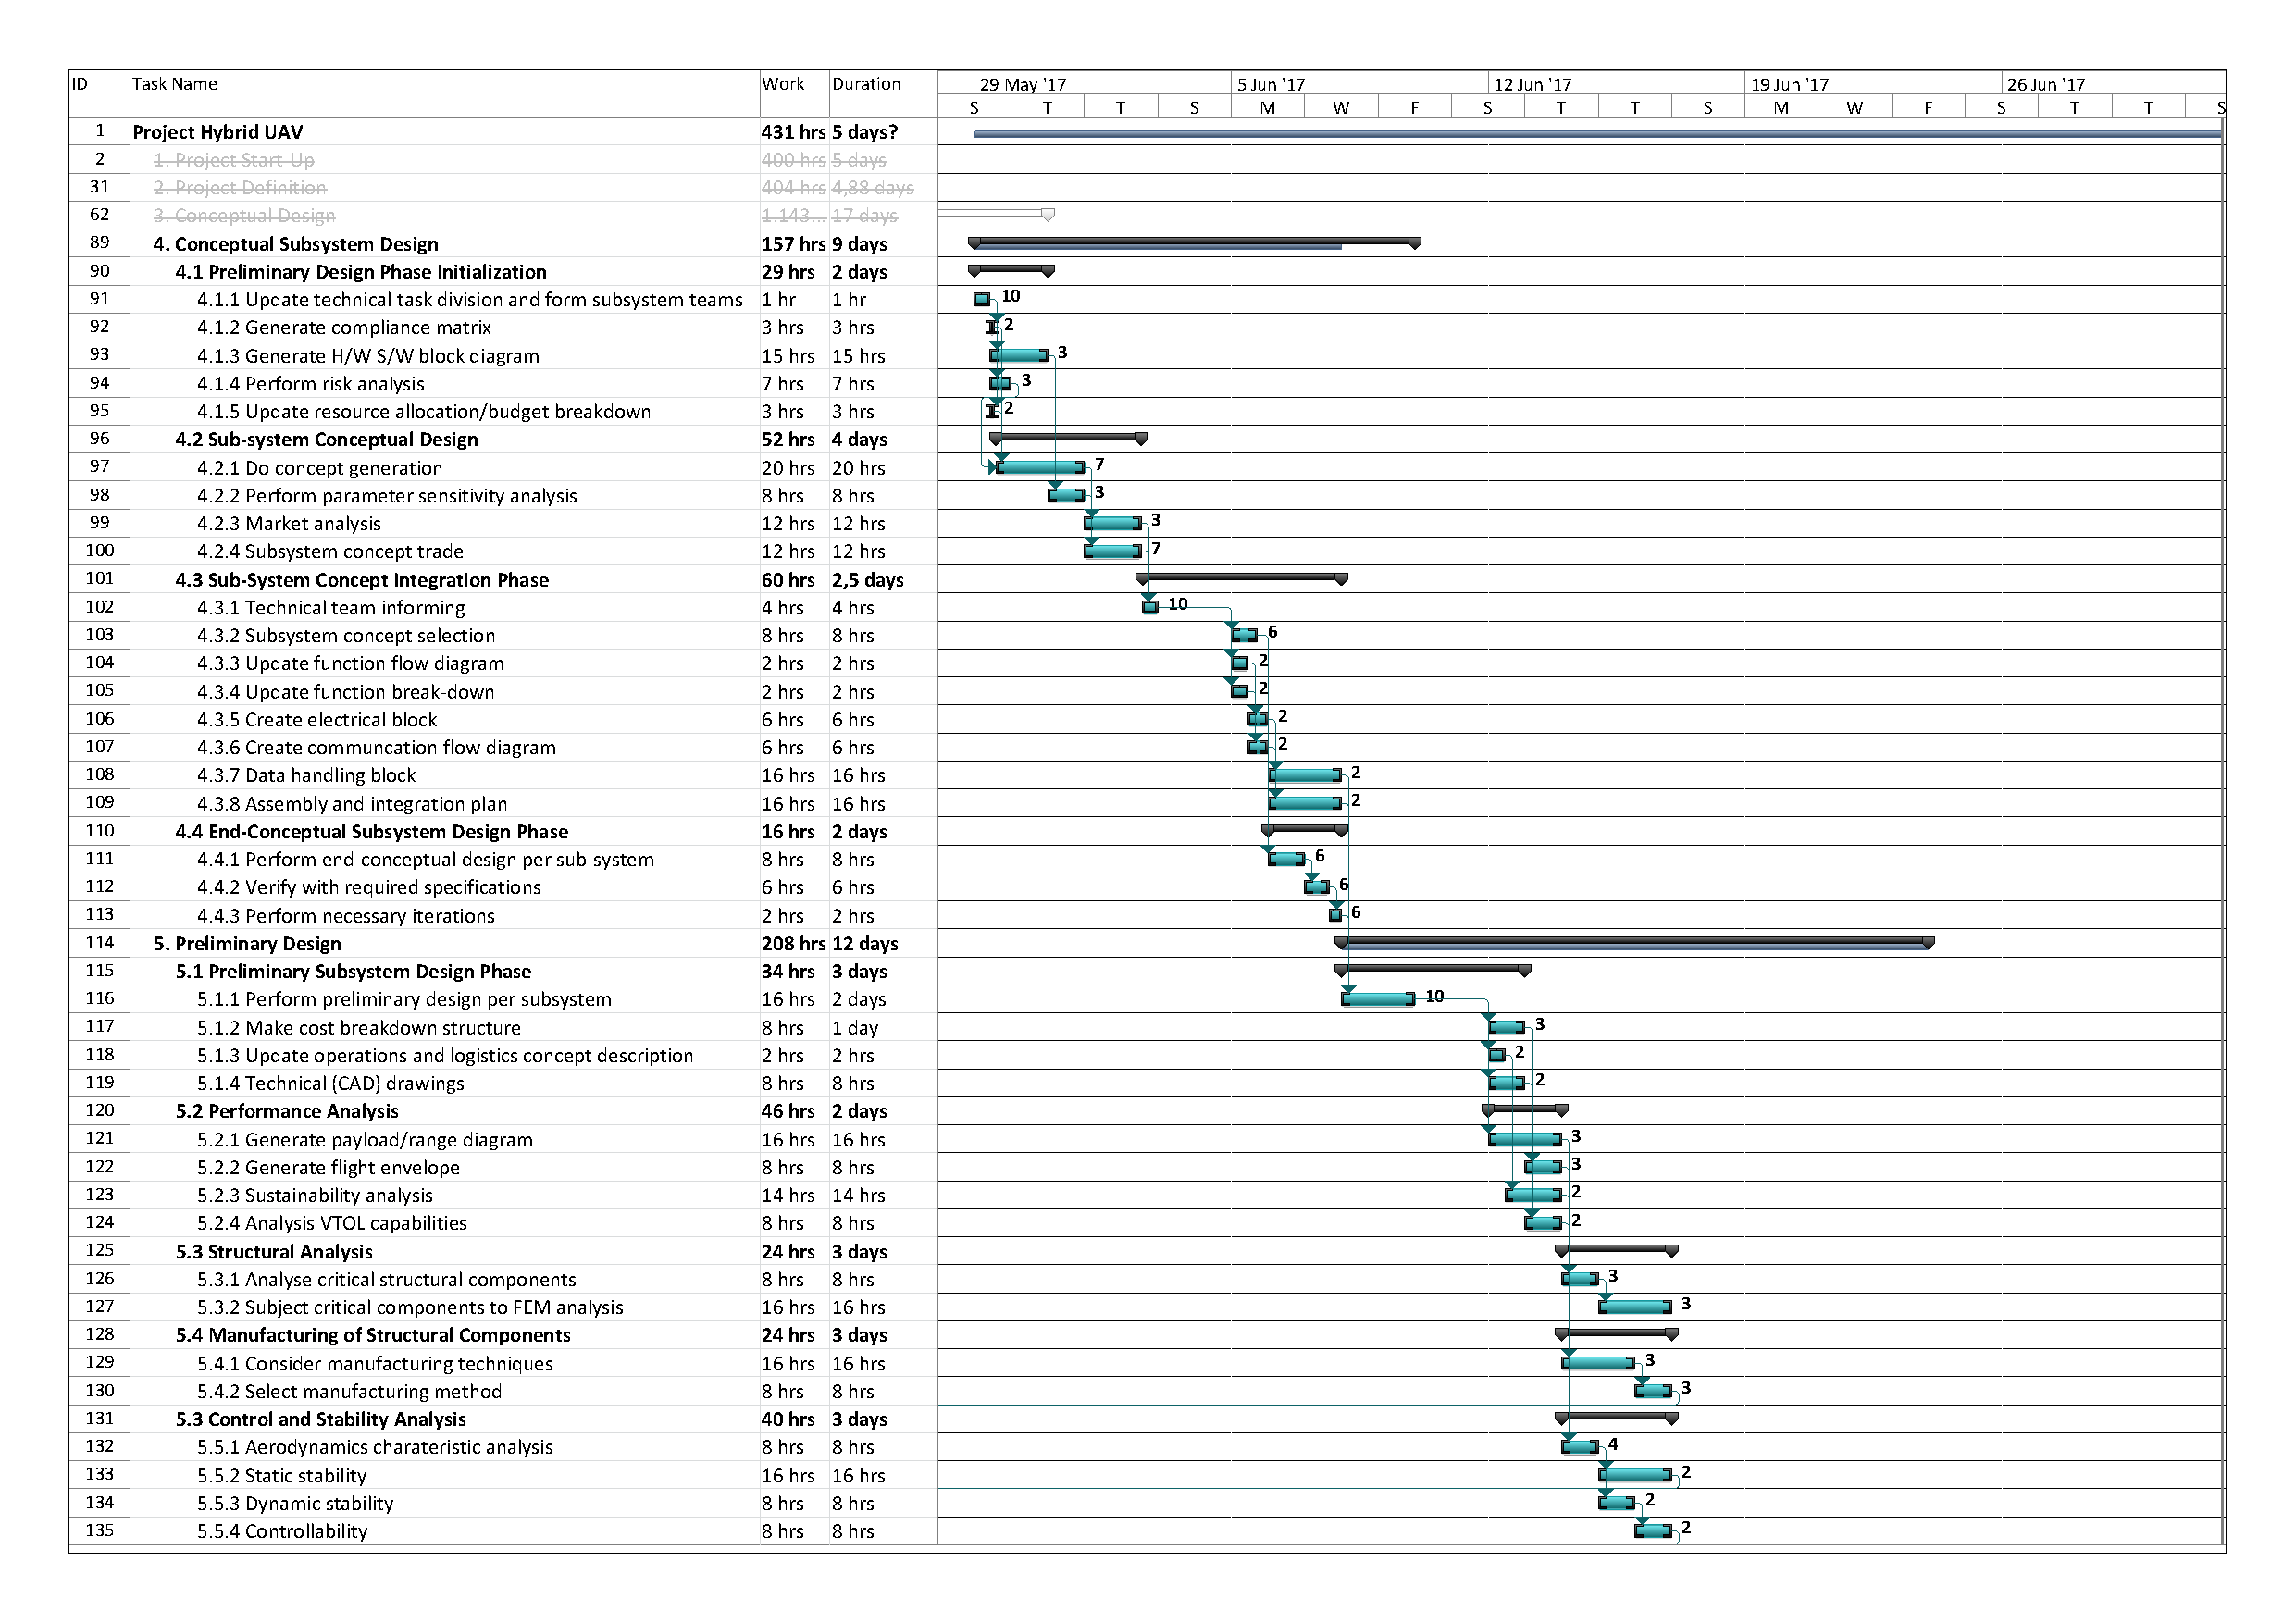
\includepdf[pages=1,fitpaper, scale=0.85,pagecommand={}]{ProjectOrganisation/Figures/Gantt_Final.pdf}

%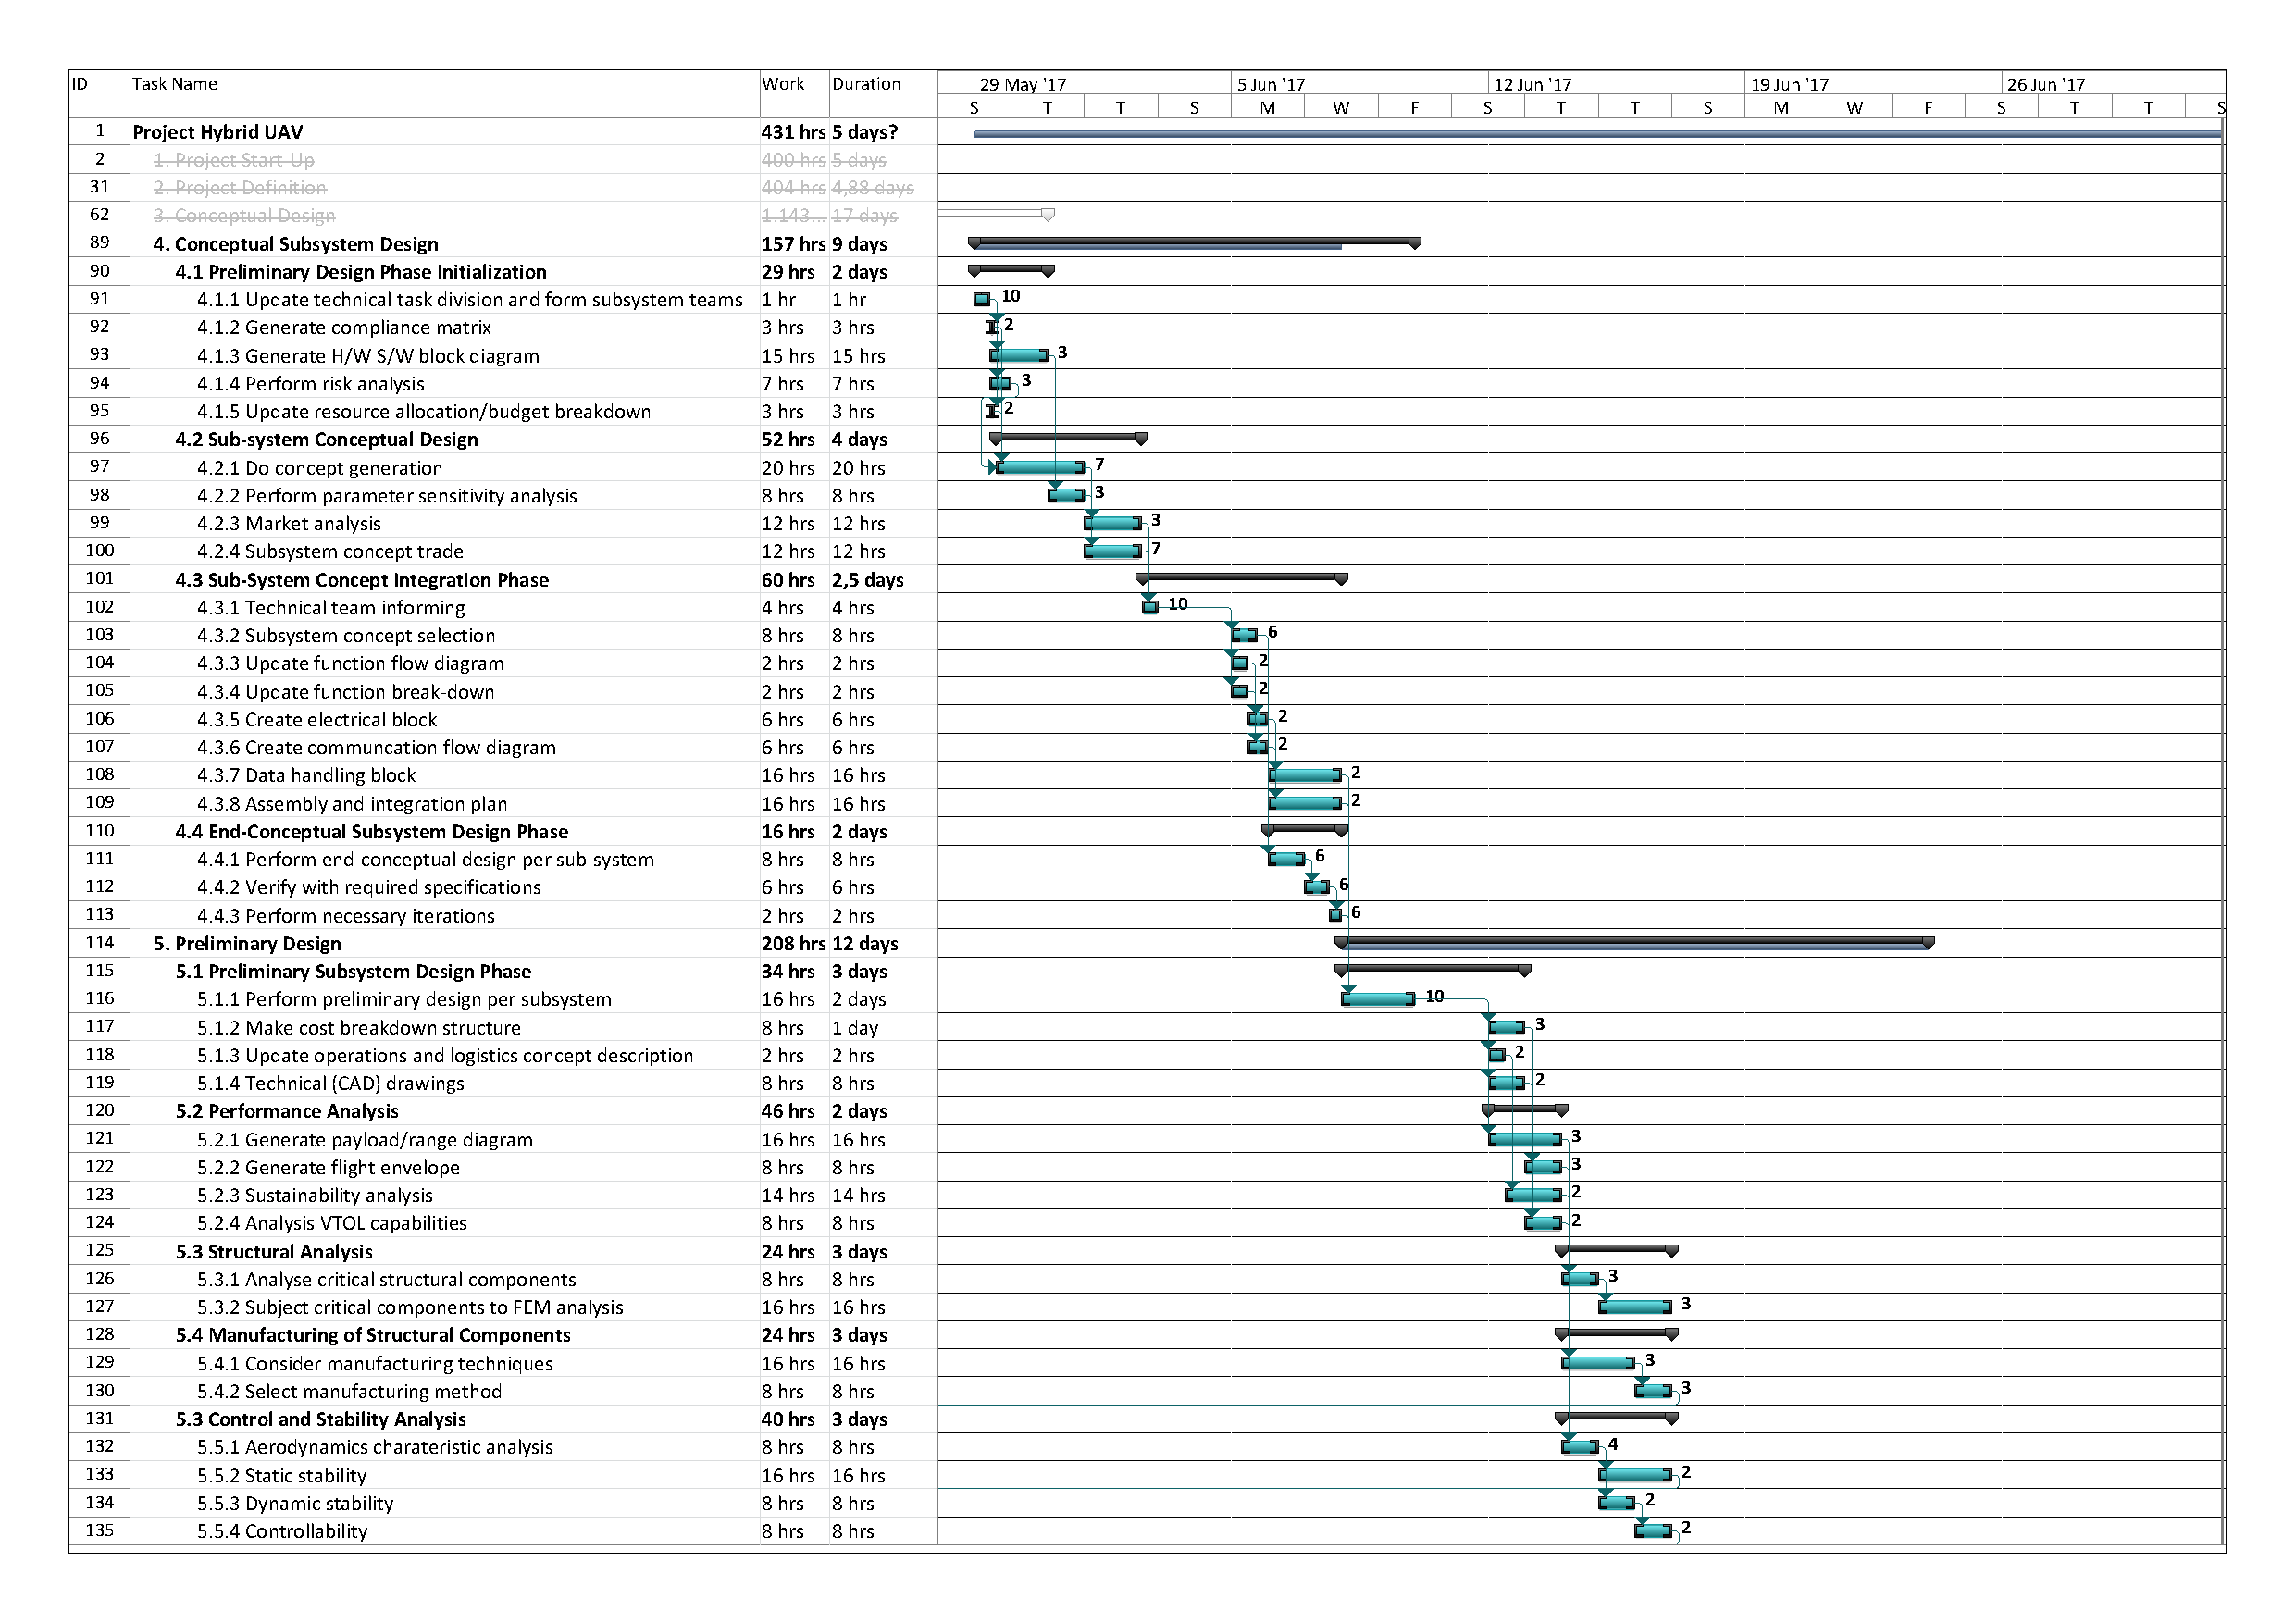
\includepdf[pages=1,fitpaper, scale=0.85,pagecommand={}]{ProjectOrganisation/Figures/Gantt_Final1.pdf}

%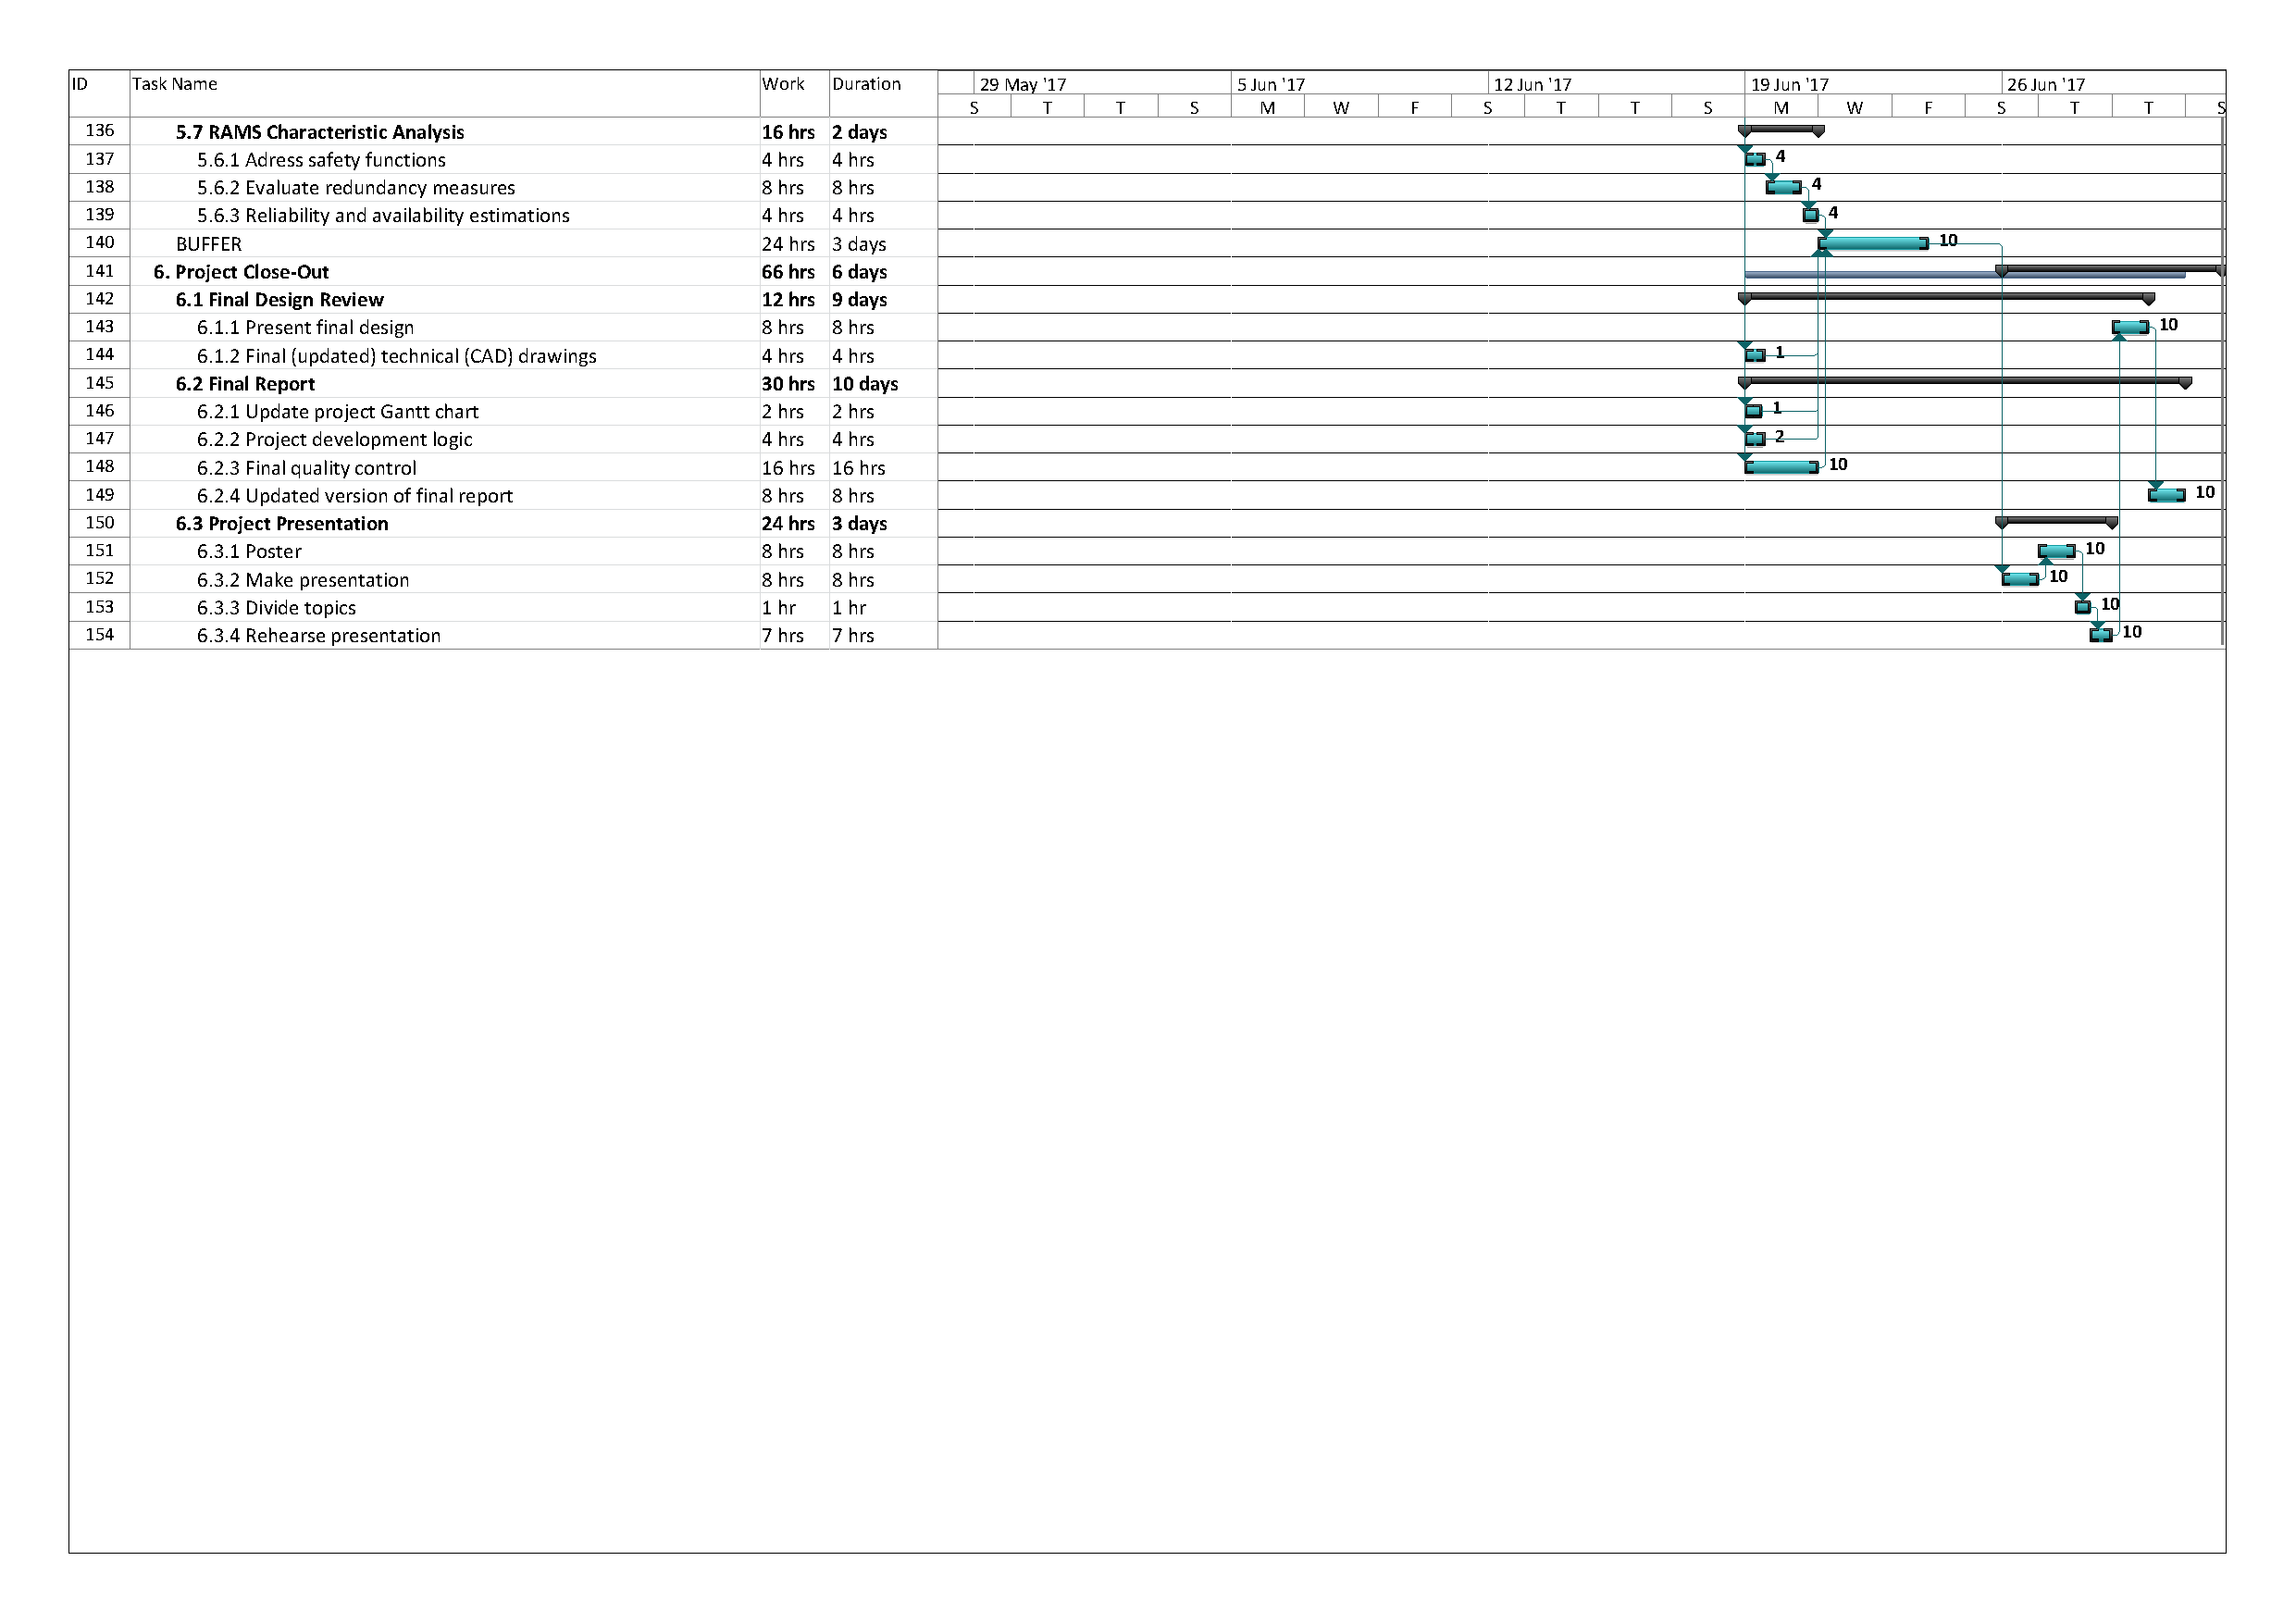
\includepdf[pages=1,fitpaper, scale=0.85,pagecommand={}]{ProjectOrganisation/Figures/Gantt_Final2.pdf}

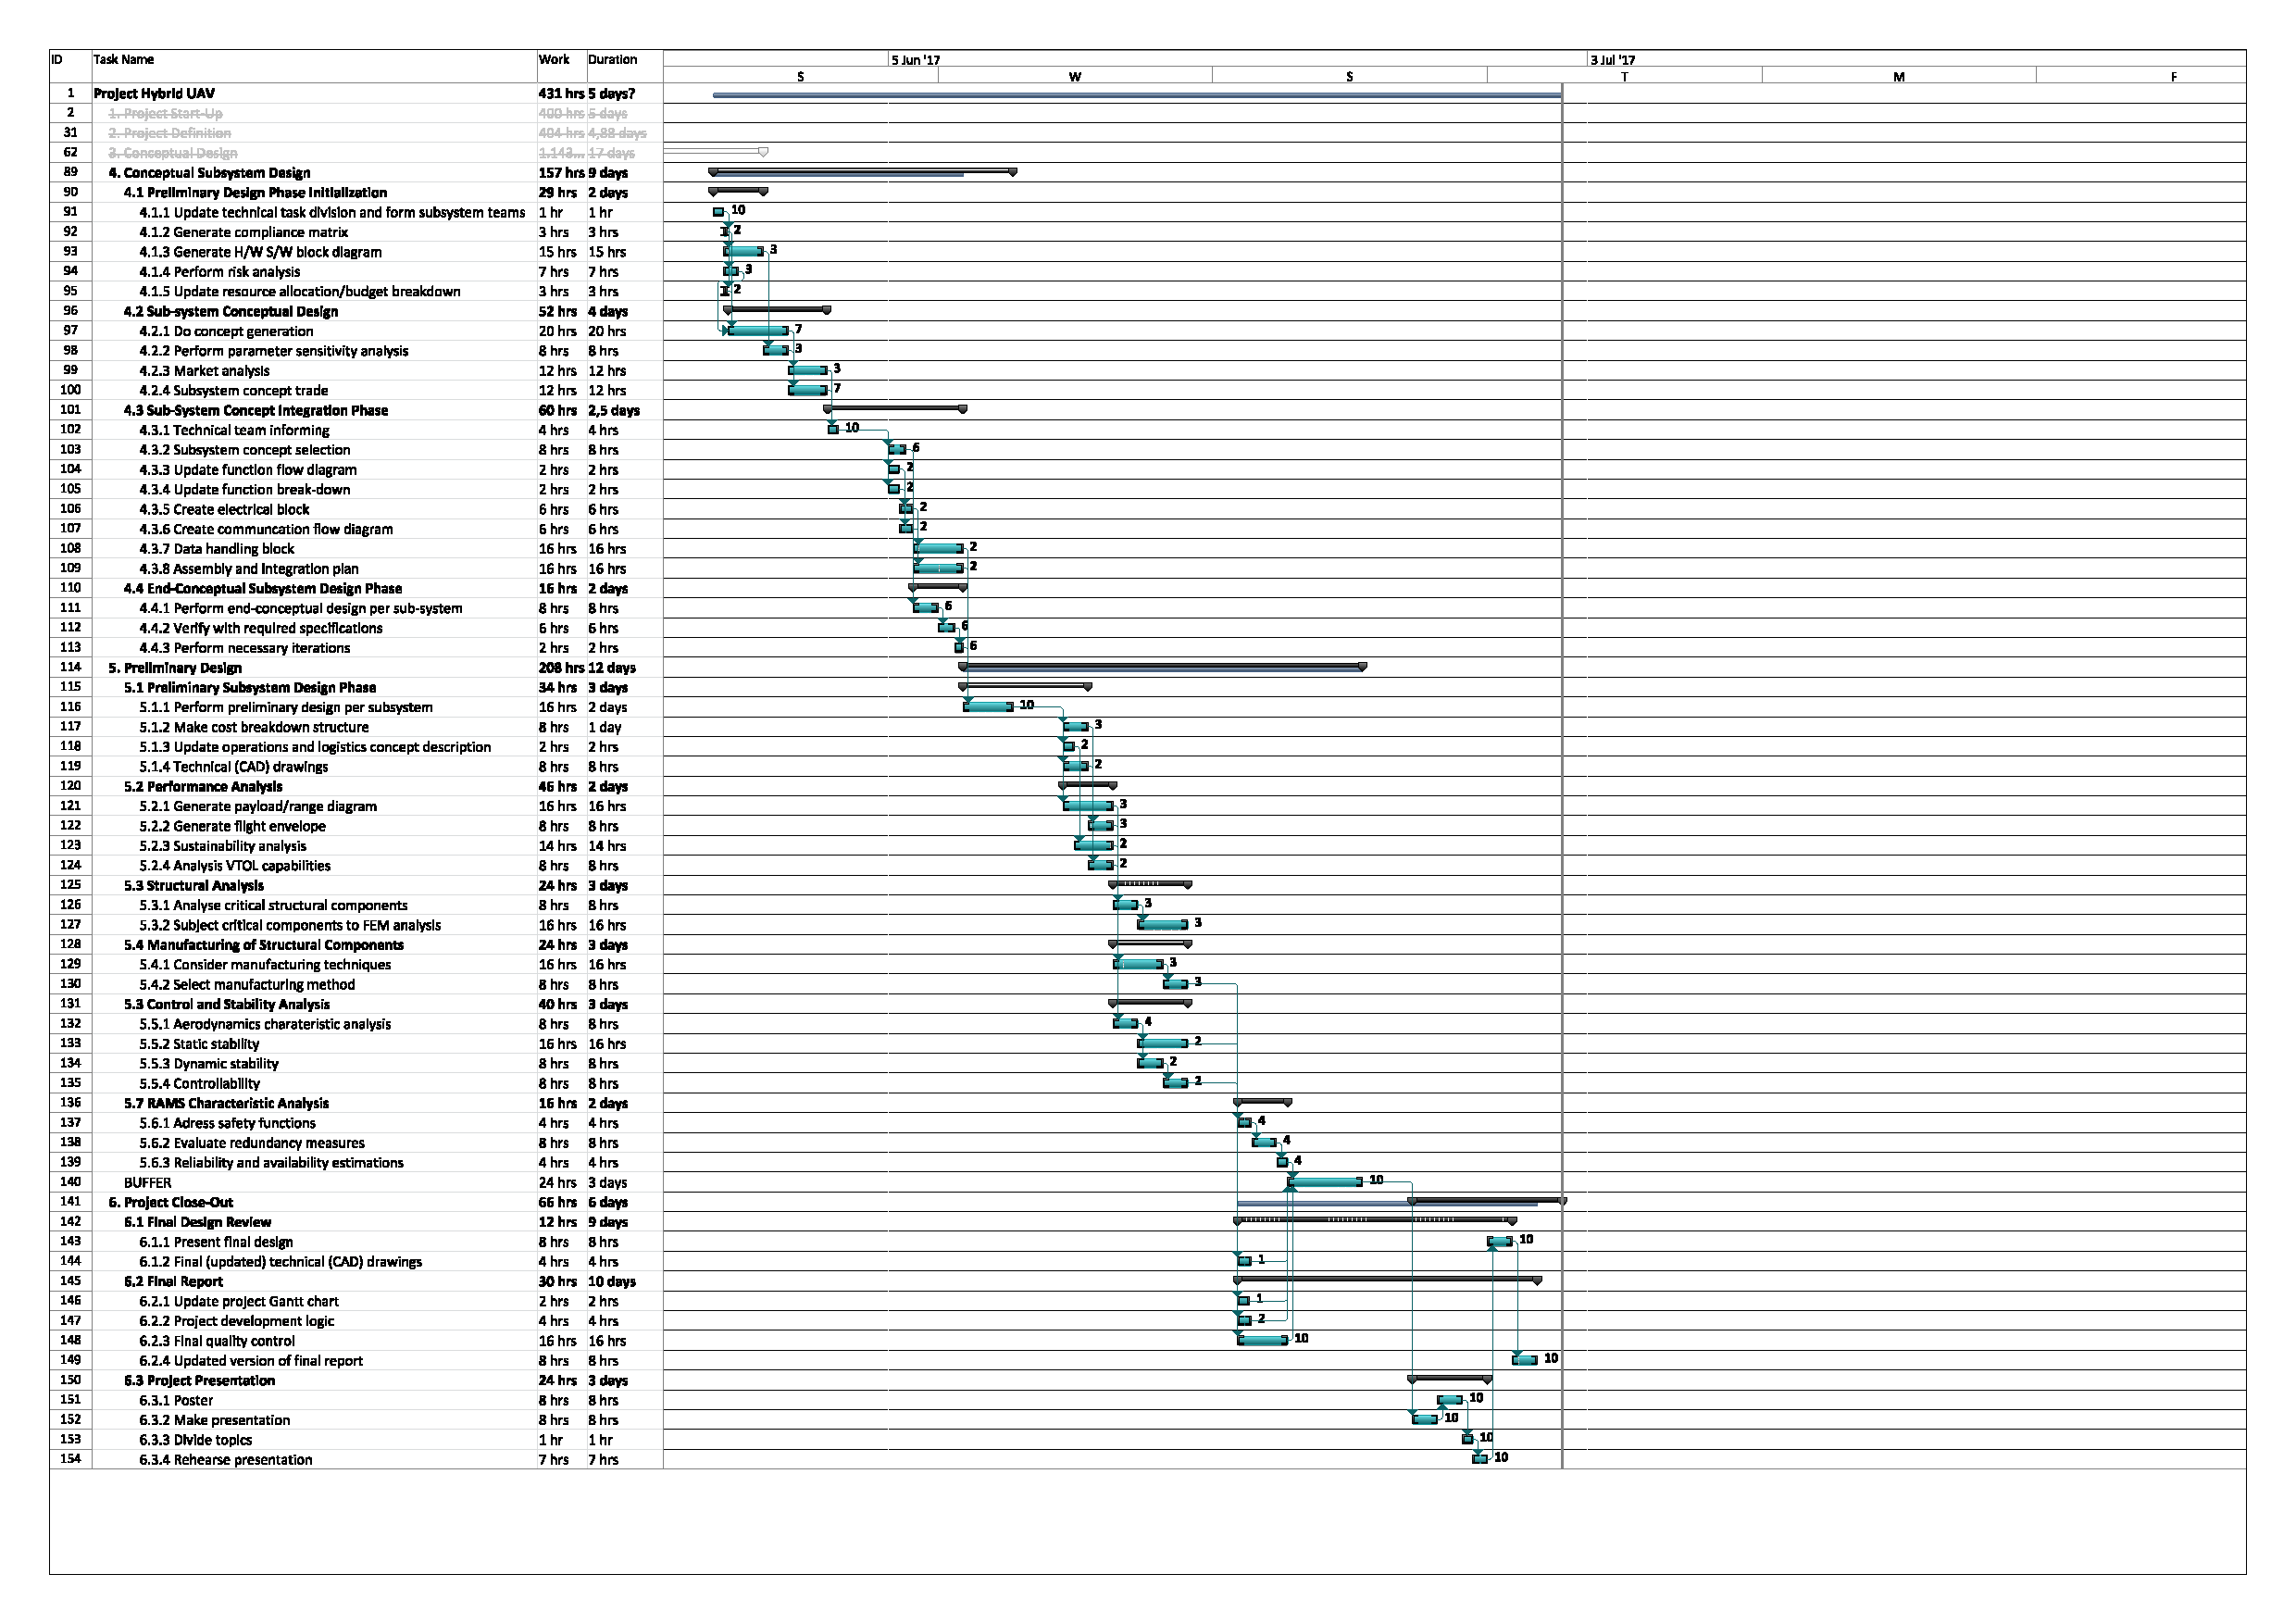
\includepdf[pages=1,fitpaper, scale=0.85,pagecommand={}]{ProjectOrganisation/Figures/gantt_small.pdf}